%ME800401
%Module 1:
%Graphs and level sets, vector fields, the tangent space, surfaces, vector fields on surfaces, orientation.
%(Chapters 1 to 5 of \cite{thorpe}) (20 hours)
%Module 2:
%The Gauss map, geodesics, Parallel transport,
%(Chapters 6, 7 & 8 of \cite{thorpe}) (20 hours)
%Module 3:
%The Weingarten map, curvature of plane curves, Arc length and line integrals
%(Chapters 9, 10 & 11 of \cite{thorpe}) (25 hours)
%Module 4:
%Curvature of surfaces and Parametrized surfaces
%(Chapters 12 & 14 of \cite{thorpe}) (25 hours)

%Module 1 - \cite{thorpe} 1, 2, 3, 4, 5
%Module 2 - \cite{thorpe} 6, 7, 8
%Module 3 - \cite{thorpe} 9, 10, 11
%Module 4 - \cite{thorpe} 12, 14
%Missing - 13, 15, 16?

%\chapter{Graphs and Level Sets}
\section{Graphs and Level Set}
\begin{definition}
	Let function $f : U \to \mathbb{R}$ where $U \subset \mathbb{R}^{n+1}$.
	Let $c$ be a real number.
	Then the \textbf{Level set} of $f$ at height $c$ is the set of all points in $U$ with image $c$.
	\begin{equation}
		f^{-1}(c) = \{ (x_1,x_2,\cdots,x_{n+1}) \in U : f(x_1,x_2,\cdots,x_{n+1}) = c \}
	\end{equation} 
\end{definition}

\begin{definition}
	Let function $f : U \to \mathbb{R}$ where $U \subset \mathbb{R}^{n+1}$.
	Then,
\begin{equation}
	graph(f) = \{ (x_1,x_2,\cdots,x_{n+2}) \in \mathbb{R}^{n+2} : f(x_1,x_2,\cdots,x_{n+1}) = x_{n+2} \}
\end{equation}
\end{definition}

\begin{figure}[h]
	\centering
	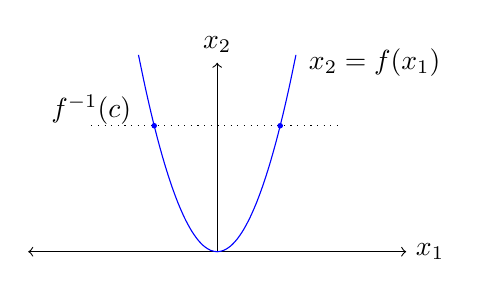
\begin{tikzpicture}[scale=0.8]
		\draw[<->] (-3, 0) -- (3, 0) node[right] {$x_1$};
  		\draw[->] (0, 0) -- (0, 3) node[above] {$x_2$};
  		\draw[scale=0.5, domain=-2.5:2.5, smooth, variable=\x, blue] plot ({\x}, {\x*\x});
		\draw[dotted,thin,black] (-2,2) -- (2,2);
		\draw (-2,2.25) node{$f^{-1}(c)$};
		\draw (2.5,3) node{$x_2 = f(x_1)$};
		\node[circle,fill=blue,inner sep=0pt, minimum size=2pt] at (1,2){};
		\node[circle,fill=blue,inner sep=0pt, minimum size=2pt] at (-1,2){};
\end{tikzpicture}
	\caption{Graph of $f(x_1)=x_1^2$ and Level set $f^{-1}(c)$}
\end{figure}

%\chapter{Vector Fields}
\section{Vector Fields}
\begin{definition}
	A vector $\mathbf{v}$ at a point $p \in \mathbb{R}^{n+1}$ is a pair $\mathbf{v} = (p,v)$ where $v \in \mathbb{R}^{n+1}$.
\end{definition}
\begin{description}
	\item[vector addition] $\mathbf{v} + \mathbf{w} = (p,v) + (p,w) = (p,v+w)$.
	\item[scalar multiplication] Let $c \in \mathbb{R}$, then $c \mathbf{v} =  c(p,v) = (p,cv)$.
	\item[dot product] $\mathbf{v}\cdot \mathbf{w} = (p,v)\cdot(p,w) = v \cdot w$
	\item[cross product] $\mathbf{v}\times \mathbf{w} = (p,v)\times(p,w) = (p,v \times w)$
\end{description}
\begin{remark}
	Angle $\theta$ between $\mathbf{v}$ and $\mathbf{w}$ is given by,
	\begin{equation}
		\cos \theta = \mathbf{v}\cdot\mathbf{w} = (p,v)\cdot(p,w) = v.w
	\end{equation}
	And the length of a vector $\mathbf{v}$ is given by,
	\begin{equation}
		\|\mathbf{v}\| = \mathbf{v}\cdot\mathbf{v} = (p,v)\cdot(p,v) = v\cdot v = \| v \|
	\end{equation}
\end{remark}

\begin{remark}
	Let $c \in \mathbb{R}$ and $p \in \mathbb{R}^{n+1}$. Let $\mathbf{v}, \mathbf{w}$ be two vectors at $p$. That is, $\mathbf{v} = (p,v)$ and $\mathbf{w} = (p,w)$ for some $v,w \in \mathbb{R}^{n+1}$. Then the set of all vectors at $p$ is a vector space with vector addition $\mathbf{v}+\mathbf{w} = (p,v+w)$ and scalar multiplication $c\mathbf{v} = (p,cv)$. This vector space is denoted by $\mathbb{R}_p^{n+1}$.
\end{remark}

\begin{figure}[h]
	\centering
	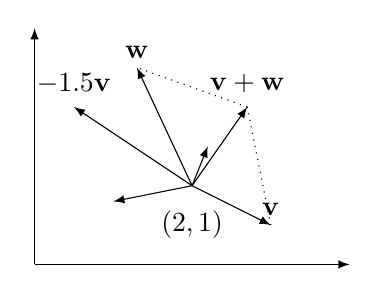
\begin{tikzpicture}
		\draw[-latex] (0,0) -- (0,3);
		\draw[-latex] (0,0) -- (4,0);

		\draw[-latex] (2,1) -- (1,0.8);
		\draw[-latex] (2,1) -- (2.2,1.5);
		%\draw[-latex] (2,1) -- (3,1.25);
		\draw[-latex] (2,1) -- (1.3,2.5); %w
		\draw[-latex] (2,1) -- (3,0.5); %v
		\draw[-latex] (2,1) -- (2.7,2); %v+w
		\draw[-latex] (2,1) -- (0.5,2); %1.5v
		\draw[dotted,thin] (3,0.5) -- (2.7,2);
		\draw[dotted,thin] (2.7,2)-- (1.3,2.5);

		\draw (2,0.5) node{$(2,1)$};
		\draw (3,0.7) node{$\mathbf{v}$};
		\draw (1.3,2.7) node{$\mathbf{w}$};
		\draw (2.7,2.3) node{$\mathbf{v+w}$};
		\draw (0.5,2.3) node{$-1.5\mathbf{v}$};
	\end{tikzpicture}
	\caption{The vector space of all vectors at $(2,1)$, $\mathbb{R}_{(2,1)}^2$}
\end{figure}

\begin{definition}
	The vector field $\mathbf{X}$ on $\mathbb{R}^{n+1}$ is a function which assigns to each point of $\mathbb{R}^{n+1}$ a vector at that point.
	That is, $\mathbf{X}(p) = (p,X(p))$.
\end{definition}

For example, $\mathbf{X}(p) = (p,X(p))$ where the associated function of the vector field, $X : \mathbb{R}^2 \to \mathbb{R}^2$ defined by $X(p) = (1,2)$ assigns a constant vector $(1,2)$ at every vector in $\mathbb{R}^2$.

\begin{figure}[h]
	\centering
	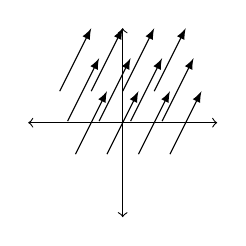
\begin{tikzpicture}[scale=0.4]
		\draw[<->] (-3,0) -- (3,0);
		\draw[<->] (0,-3) -- (0,3);

		\draw[-latex] (1,1) -- (2,3);
		\draw[-latex] (0,1) -- (1,3);
		\draw[-latex] (-1,1) -- (0,3);
		\draw[-latex] (-2,1) -- (-1,3);

		\draw[-latex] (1.25,0.05) -- (2.25,2.05);
		\draw[-latex] (0.25,0.05) -- (1.25,2.05);
		\draw[-latex] (-0.75,0.05) -- (0.25,2.05);
		\draw[-latex] (-1.75,0.05) -- (-0.75,2.05);

		\draw[-latex] (1.5,-1) -- (2.5,1);
		\draw[-latex] (0.5,-1) -- (1.5,1);
		\draw[-latex] (-0.5,-1) -- (0.5,1);
		\draw[-latex] (-1.5,-1) -- (-0.5,1);

	\end{tikzpicture}
	\caption{Vector field with associated function $X(p) = (1,2)$}
\end{figure}

\begin{definition}[smooth]
	A function $f : \mathbb{R} \to \mathbb{R}$ is smooth if its partial derivatives of all orders exists and are continuous.
	A function $f : \mathbb{R}^{n+1} \to \mathbb{R}$ is smooth if its component functions $f = (f_1, f_2, \cdots, f_{n+1})$ are smooth.
	A vector field $\mathbf{X}$ is smooth if the associated function $X(p)$ is smooth.
\end{definition}

\begin{definition}
	Let $f : \mathbb{R}^{n+1} \to \mathbb{R}$. Then the gradient of $f$ at $p$ is,
	\begin{equation}
		\nabla f(p) = \left(p,\frac{\partial f}{\partial x_1}(p),\frac{\partial f}{\partial x_2}(p),\cdots,\frac{\partial f}{\partial x_{n+1}}(p)\right)
	\end{equation}
\end{definition}

\begin{remark}
	If $f$ is a smooth function, then the gradient of $f$ at $p$ is a smooth vector field.
\end{remark}
	For example, $f : \mathbb{R}^2 \to \mathbb{R}$ defined by $f(x_1,x_2) = 2x_1x_2$ is a smooth function. We have, $\frac{\partial f}{\partial x_1} = 2x_2$ and $\frac{\partial f}{\partial x_2} = 2x_1$. And gradient of $f$ at $(x_1,x_2)$ is $(x_1,x_2,2x_2,2x_1)$. That is, $(2x_2,2x_1)$ at $(x_1,x_2)$.

Calculations : \\
\begin{tabular}{|c|c|c|c|c|c|c|} \hline
	$p$    & $(x_1,x_2)$   & $(0,0)$ & $(1,0)$ & $(0,1)$ & $(-1,0)$ & $(0,-1)$ \\ \hline
	$X(p)$ & $(2x_2,2x_1)$ & $(0,0)$ & $(0,2)$ & $(2,0)$ & $(0,-2)$ & $(-2,0)$ \\ \hline
\end{tabular}

\begin{figure}[h]
	\centering
	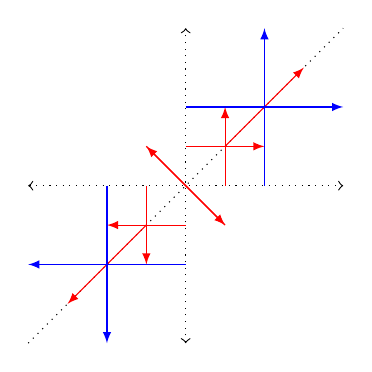
\begin{tikzpicture}[scale=0.5]
		\draw[<->,dotted] (0,-4) -- (0,4);
		\draw[<->,dotted] (-4,0) -- (4,0);
		\draw[dotted] (-4,-4) -- (4,4);

		\draw[-latex,color=red] (1,1) -- (3,3);
		\draw[-latex,color=red] (-1,1) -- (1,-1);
		\draw[-latex,color=red] (1,-1) -- (-1,1);
		\draw[-latex,color=red] (-1,-1) -- (-3,-3);
		\draw[-latex,color=red] (0,1) -- (2,1);
		\draw[-latex,color=red] (0,-1) -- (-2,-1);
		\draw[-latex,color=red] (1,0) -- (1,2);
		\draw[-latex,color=red] (-1,0) -- (-1,-2);

		%\draw[-latex] (-1,2) -- (3,0);
		%\draw[-latex] (2,-1) -- (0,3);
		%\draw[-latex] (1,-2) -- (-3,0);
		%\draw[-latex] (-2,1) -- (0,-3);

		\draw[-latex,color=blue] (0,2) -- (4,2);
		\draw[-latex,color=blue] (2,0) -- (2,4);
		\draw[-latex,color=blue] (-2,0) -- (-2,-4);
		\draw[-latex,color=blue] (0,-2) -- (-4,-2);

		%\draw[-latex] (1,0.5) -- (2,2.5);
		%\draw[-latex] (0.5,1) -- (2.5,2);
		%\draw[-latex] (-1,0.5) -- (0,-1.5);
		%\draw[-latex] (0.5,-1) -- (-1.5,0);
		%\draw[-latex] (1,-0.5) -- (0,1.5);
		%\draw[-latex] (-0.5,1) -- (1.5,0);
		%\draw[-latex] (-1,-0.5) -- (-2,-2.5);
		%\draw[-latex] (-0.5,-1) -- (-2.5,-2);
	\end{tikzpicture}
	\caption{The gradient of $f(x_1,x_2) = 2x_1x_2$}
\end{figure}

\begin{definition}
	A parameterised curve is a function, $\alpha : I \to \mathbb{R}^{n+1}$ where $I$ is some open interval in $\mathbb{R}$.
	The velocity vector of a parameterised curve $\alpha : I \to \mathbb{R}^{n+1}$ at a point $\alpha(t)$ is the tangent to the curve at that point.
	\begin{equation}
		\dot{\mathbf{\alpha}}(t) = \left(\alpha(t),\frac{d \alpha}{dt} (t)\right)
	\end{equation}
\end{definition}

For example, $\alpha : I \to \mathbb{R}^2$ defined by $\alpha(t) = (2t,t^2)$ is a parameterised curve. We have, $\frac{d\alpha}{dt} = (\frac{dx_1}{dt}(t),\frac{dx_2}{dt}(t)) = (2,2t)$ where $\alpha(t) = (x_1(t),x_2(t))$. The velocity vector at $t = 3$ is $\dot{\alpha}(3) = (\alpha(t),\frac{d\alpha}{dt}) = (6,9,2,6)$.

\begin{definition}
	Let $\mathbf{X}$ be a vector field and let $U$ be an open subet of $\mathbb{R}^{n+1}$.
	An integral curve $\alpha$ on $U$ is a parameterised curve, $\alpha : I \to \mathbb{R}^{n+1}$ such that for each $\alpha(t) = p \in U$, the velocity vector $\dot{\alpha}(t)$ is the associated vector $\mathbf{X}(p)$ of the vector field $\mathbf{X}$ at that point. Thus, for each $t \in I$, $\dot{\alpha}(t) = \mathbf{X}(\alpha(t))$.
	\begin{equation}
		\left(\alpha(t),\frac{d \alpha}{dt}(t)\right) = \left(\alpha(t),X(\alpha(t))\right)
	\end{equation}
	Let $X(p) = \left(X_1(p),X_2(p),\cdots,X_{n+1}(p)\right)$ and $\alpha(t) = \left(x_1(t),x_2(t),\cdots,x_{n+1}(t)\right)$. Then, comparing components of the vector at $\alpha(t)$ we get the following system of equations,
	\begin{equation}
		\frac{d x_j}{dt}(t) = X_j(\alpha(t)),\ j = 1,2,\cdots,(n+1)
	\end{equation}
\end{definition}

For example, Consider $\alpha : (2,3) \to \mathbb{R}^2$ defined by $\alpha(t) = (t,t^2)$. Then $\alpha$ is a parameterised curve in vector field, $\mathbf{X}$ which has the associated function $X(x_1,x_2) = (1,2x_1)$. Then, $\mathbf{X}(x_1,x_2) = (x_1,x_2,1,2x_1)$. And
\[ \dot{\alpha}(t) = \left( \alpha(t),\frac{d\alpha}{dt}(t) \right) = \left( x_1(t),x_2(t),\frac{dx_1}{dt}(t), \frac{dx_2}{dt}(t) \right) = (t,t^2,1,2t) \]
Clearly, $\alpha$ is an integral curve of $\mathbf{X}$ as $\dot{\alpha}(t) = X(\alpha(t))$ for every $t \in (2,3)$.

Calculations:\\
\begin{tabular}{|c|c|c|c|c|c|c|c|c|c|} \hline
	$p$    & $(0,0)$ & $(1,0)$ & $(0,1)$ & $(1,1)$ & $(-1,0)$ & $(0,-1)$ & $(-1,1)$ & $(1,-1)$ & $(-1,-1)$ \\ \hline
	$X(p)$ & $(1,0)$ & $(2,2)$ & $(1,1)$ & $(2,3)$ & $(0,-2)$ & $(1, 1)$ & $(0,-1)$ & $(2, 1)$ & $( 0,-3)$ \\ \hline
\end{tabular}

\begin{figure}[h]
	\centering
	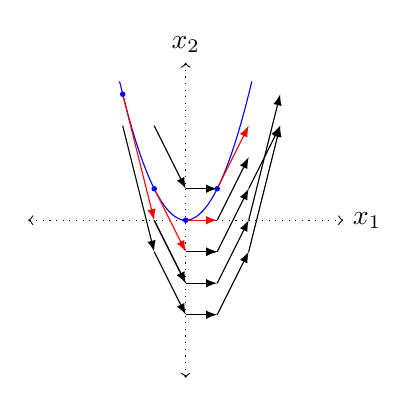
\begin{tikzpicture}[scale=0.4]
		\draw[<->,dotted] (-5, 0) -- (5, 0) node[right] {$x_1$};
  		\draw[<->,dotted] (0,-5) -- (0, 5) node[above] {$x_2$};
  		\draw[domain=-2.1:2.1, smooth, variable=\x, blue] plot ({\x}, {\x*\x});

		\draw[-latex,color=red] (0,0) -- (1,0);

		\draw[-latex] (0,1) -- (1,1);
		\draw[-latex] (1,0) -- (2,2);
		\draw[-latex] (-1,3) -- (0,1);

		\draw[-latex,color=red] (-2,4) -- (-1,0);
		\draw[-latex,color=red] (1,1) -- (2,3);

		\draw[-latex] (0,-1) -- (1,-1);
		\draw[-latex,color=red] (-1,1) -- (0,-1);

		\draw[-latex] (-1,0) -- (0,-2);
		\draw[-latex] (0,-2) -- (1,-2);
		\draw[-latex] (1,-2) -- (2,0);
		\draw[-latex] (2,0) -- (3,4);

		\draw[-latex] (0,-1) -- (1,-1);
		\draw[-latex] (-1,0) -- (0,-2);

		\draw[-latex] (-2,3) -- (-1,-1);
		\draw[-latex] (-1,-1) -- (0,-3);
		\draw[-latex] (0,-3) -- (1,-3);
		\draw[-latex] (1,-3) -- (2,-1);
		\draw[-latex] (2,-1) -- (3,3);

		\draw[-latex] (0,-1) -- (1,-1);
		\draw[-latex] (1,-1) -- (2,1);
		\draw[-latex] (2,1) -- (3,3);

		\node[circle,fill=blue,inner sep=0pt, minimum size=2pt] at (1,1){};
		\node[circle,fill=blue,inner sep=0pt, minimum size=2pt] at (0,0){};
		\node[circle,fill=blue,inner sep=0pt, minimum size=2pt] at (-1,1){};
		\node[circle,fill=blue,inner sep=0pt, minimum size=2pt] at (-2,4){};
\end{tikzpicture}
	\caption{Integral Curve $\alpha(t) = (t,t^2)$ in $\mathbf{X}$ with $X(x_1,x_2) = (1,2x_1)$}
\end{figure}

\begin{theorem}
	Let $\mathbf{X}$ be a smooth vector field on an open set $U \subset \mathbb{R}^{n+1}$ and let $p \in U$.
	Then there exists an open interval $I$ containing $0$ and an integral curve $\alpha : I \to U$ such that
	\begin{enumerate}
		\item $\alpha(0) = p$
		\item If $\beta : \tilde{I} \to U$ is any other integral curve with $\beta(0) = p$, then $\tilde{I} \subset I$ and $\beta(t) = \alpha(t)$, for all $t \in \tilde{I}$.
	\end{enumerate}
\end{theorem}
\begin{proof}
	Let $\mathbf{X}$ be a smooth vector field.
	Suppose $\alpha$ be an integral curve in $\mathbf{X}$.
	Then, $\dot{\alpha}(t) = \mathbf{X}(\alpha(t))$.
	Let $x_j(t)$ be the components of $\alpha(t)$ and $X_j(p)$ be the components of $X(p)$.
	\begin{align*}
		\dot{\alpha}(t) & = \left(\alpha(t),\frac{d \alpha}{dt}(t)\right) \\
		& = \left(x_1(t),\cdots,x_{n+1}(t),\frac{dx_1}{dt}(t),\cdots,\frac{dx_{n+1}}{dt}(t)\right)\\
		\mathbf{X}(\alpha(t)) & = (\alpha(t),X(\alpha(t))) \\
		& = \left( x_1(t),\cdots,x_{n+1}(t),X_1(\alpha(t)),\cdots,X_{n+1}(\alpha(t))\right)
	\end{align*}
	Thus, we a system of $n+1$ first order differential equations in $n+1$ unknowns satisfying the initial condition $\alpha(0) = p$.
	\begin{align*}
		\frac{dx_1}{dt}(t) & = X_1(\alpha(t)) \\
		\frac{dx_2}{dt}(t) & = X_2(\alpha(t)) \\
		& \vdots \\
		\frac{dx_{n+1}}{dt}(t) & = X_{n+1}(\alpha(t))
	\end{align*}
\end{proof}
	By the theorem on solution of systems of first order ordinary differential equations, there exists an interval $I$ containing $0$ and a solution --- a family of functions $\{ x_1(t), x_2(t), \cdots,x_{n+1}(t)\}$ satisfying the above system of equations satisfying the initial condition $\alpha(0) = p$.

	Define $\alpha : I \to U$ using the component functions of $\alpha$ as $x_j$s in the above solution. Then, we have a integral curve of the vector field $\mathbf{X}$ satifying the initial condition $\alpha(0) = p$.

	Let $\beta : \tilde{I} \to U$ be another integral curve with $\beta(0) = p$. Then by the uniqueness of the solution for the system of first order ordinary differential equations with an initial condition, $\beta(t) = \alpha(t)$ for every $ t \in I \cup \tilde{I}$.

	Let $\{\beta_1,\beta_2,\cdots\}$ be the family of integral curves with $\beta_j : I_j \to U$ satisfying $\beta_j(0) = p$. Consider $I = \bigcup\limits_{j \in \mathbb{N}} I_j$.

	Define $\alpha : I \to U$ by $\alpha(t) = \beta_j(t)$ where $t \in I_j$ for some $j \in \mathbb{N}$. Then $\alpha$ is well-defined and is a maximal integral curve in $\mathbf{X}$ such that $\alpha(0) = p$.

\begin{definition}
	A smooth vector field $\mathbf{X}$ on $U \subset \mathbb{R}^{n+1}$ is \textbf{complete} if for every $p \in U$, the maximal integral curve through $p$ has domain equal to $\mathbb{R}$.
\end{definition}

\begin{definition}
	The \textbf{divergence} of a smooth vector field $\mathbf{X}$ on $U \subset \mathbb{R}^{n+1}$ is the function $div\ \mathbf{X} : U \to \mathbb{R}$ defined by
	\[ div\ X(x_1,x_2,\cdots,x_{n+1}) = \sum_{i=1}^{n+1} \frac{\partial X_i}{\partial x_i} \]
	where $X_i$ are the component function of the associated function $X$ of the vector field $\mathbf{X}$.
\end{definition}

For example, Consider $\mathbf{X}$ with associated function $X : \mathbb{R}^2 \to \mathbb{R}^2$ defined by $X(x_1,x_2) = (2x_1,x_1x_2)$. Then $div\ \mathbf{X}(x_1,x_2) = \frac{\partial X_1}{\partial x_1} + \frac{\partial X_2}{\partial x_2} = 2 + x_1$.

%\chapter{The Tangent Space}
\section{The Tangent Space}

%\chapter{Surfaces}
\section{Surfaces}

%\chapter{Vector Fields on Surfaces; Orientation}
\section{Vector Fields on Surfaces; Orientation}

%\chapter{The Gauss Map}
\section{The Gauss Map}
	Suppose $S$ is an $n$-surface. From the definition of an $n$-surface, there exists a smooth function $f : U \to \mathbb{R}$ where $U$ is an open subset of $\mathbb{R}^{n+1}$ such that $S = f^{-1}(c)$ for some real value $c \in \mathbb{R}$ and every point on $S$ is a regular point of $f$. That is $\nabla f(p) \ne \mathbf{0}$ for every point $p$ on the surface $S$.\\

	We have proved that every $n$-surface has exactly two orientations $\mathbf{N}_1$ and $\mathbf{N}_2$. These orientations are $\frac{\nabla f}{\| \nabla f\|}$ and $\frac{-\nabla f}{\| \nabla f\|}$. Given an orientation $\mathbf{N}$ (either $\mathbf{N}_1$ or $\mathbf{N}_2$), the surface together with that orientation is collectively referred as an oriented $n$-surface.\\

	\textbf{Since orientation $\mathbf{N}$ is a smooth, unit normal vector field. The vector field $\mathbf{N}$ has an associated function $N : U \to \mathbb{R}^{n+1}$. That is $\mathbf{N}(p) = (p,N(p))$ where $N : U \to \mathbb{R}^{n+1}$. And we already have, $\mathbf{N}(p) = (p,N(p)) = (p, \frac{\pm \nabla f}{\| \nabla f\|})$. This associated function restricted to the $n$-surface $S$ is the \textbf{Gauss Map}. That is, $N : S \to \mathbb{R}^{n+1}$.}\\

	From the definition of orientation, we know that this function is actually assigning direction to each point on that surface $S$. If you don't remember, the directions are vector in $\mathbb{R}^{n+1}$ of unit length. That is $\|v\| = 1$. Thus, the range of Gauss Map is a subset of the set of all directions. And unit sphere $S^n$ is $\mathbb{R}^{n+1}$ is the set of all directions in $\mathbb{R}^{n+1}$.\\

	Thus, we may write Gauss Map, $N : S \to S^n$
\subsection{Spherical Image}
	We already saw that, the Gauss Map $N : S \to S^n$ is a function which maps directions/unit vectors to each point on that oriented surface $S$.\\

	Do we need an oriented surface ? Yes. The Gauss Map is defined by this orientation. If we are provided with an oriented $n$ Surface $S$, then we have a unit vector/orientation assigned to each point $p$ on that surface. And Gauss Map assigns this unit vector to the point $p$ on surface $S$.\\

	We already saw that the range of the Gauss Map is a subset of the unit $n$ Sphere $S^n$. In other words, the Gauss Map assigns each point on the oriented $n$-surface $S$ into a subset of the unit $n$ sphere $S^n$. Thus, \textbf{range of the Gauss Map is referred as the spherical image of the oriented $n$-surface $S$}.
	\begin{equation}
	N(S) = \{ q \in S^n : q = N(p),\ p \in S \}
	\end{equation}

\subsection{Compact, connected, oriented $n$ Surface}
	Suppose we have a compact, connected, oriented $n$-surface $S$. The compact subsets in Euclidean spaces are closed and bounded subsets. And connected subsets in Euclidean Spaces are path connected.\\

\begin{theorem}[Spherical Image of Compact, Connected, Oriented Surface]
	The Gauss map of a compact, connected, oriented $n$-surface is surjective.
\end{theorem}
\begin{proof}
	Let $v \in S^n$ be a direction in $\mathbb{R}^{n+1}$. Let $S$ be a compact, connected, oriented $n$-surface with orientation $N$ such that $S = f^{-1}(c)$ and every point $p \in S$ are regulr points of the smooth function $f : U \to \mathbb{R}$ where $U$ is an open subset of $\mathbb{R}^{n+1}$. Thus, we have the Gauss Map $N: S \to S^n$ defined by the orientation on $S$.\\
	
	Since $v$ is arbitary, it is enough to prove that $v \in N(S)$. Suppose there exists $v \in S^n$ such that $v \notin N(S)$, then the Gauss Map is not surjective. In other words, $N$ is surjective if for every $v \in S^n,\ v \in N(S)$ OR for every $v \in S^n$, there exists $p \in S$ such that $v = N(p)$\\

	Let $g : \mathbb{R}^{n+1} \to \mathbb{R}$ defined by $g(p) = p \cdot v$. Then $g$ is a smooth function since first order partial derivatives are constant functions and all other partial derivatives of higher orders vanishes.\\

	Since $S$ is compact, $g$ restricted to $S$ is a continuous function defined on a compact interval. And thus it attains maximum and minimum values, say $p$ and $q$. The maximum and minimum values of the dot product $p \cdot v$ are $\pm v$.\\
	
	By Lagrange's multiplier theorem, $\nabla g(p) = \lambda \nabla f(p)$ and $\nabla g(q) = \lambda \nabla f(q)$. From the definition of the Gauss Map, we have $\nabla g(p) = \lambda \nabla f(p) = \lambda \| \nabla f(p) \| \mathbf{N}(p) = \lambda \| \nabla f(p) \| (p,v)$. Thus, $v$ and $N(p)$ are multiples of one another. Similarly, $\nabla g(q) = \lambda \| \nabla f(q) \| \mathbf{N}(q)$. Therefore $N(p) = \pm v$ and $N(q) = \pm v$.\\
	
	It remains to show that $N(p) \ne N(q)$. Suppose $N(p) = N(q)$. If there exists continuous function $\alpha$ such that $\alpha : [0,1] \to \mathbb{R}^{n+1}$, $\alpha(0) = p$, $\alpha(1) = q$, $\dot{\alpha}(0) = (p,v)$ and $\dot{\alpha}(1) = (q,v)$. And $\alpha$ maps the interior, the open interval $(0,1)$ outside the surface $S$. Then by intermediate value theorem, we arrive at a contradiction. And thus $N(p) \ne N(q)$.\\

	Let $\alpha_1 : [0,x] \to \mathbb{R}^{n+1}$ defined by $\alpha_1(t) = p+tv$. Let $\alpha_2 : [y,1] \to \mathbb{R}^{n+1}$ defined by $\alpha_2(t) = q+(t-1)v$. Let $\alpha_3 : [x,y] \to S_1$ where $S_1$ is an $n$ sphere properly containing $S$. Such an $n$ sphere exists, since $S$ is compact (bounded). And there exists such a function $\alpha_3$, the image of which is a compact subset of $S_1$.\\
	
	Now consider $\alpha : [0,1] \to \mathbb{R}^{n+1}$ defined by
	\begin{equation}
		\alpha(t) = \begin{cases} \alpha_1(t) & t \in [0,x) \\ \alpha_3(t) & t \in [x,y] \\ \alpha_2(t) & t \in (y,1] \end{cases}
	\end{equation}

\begin{figure}[hbt]
	\centering
	\begin{tikzpicture}[scale=0.6]

	\draw (2,2.5) node{$p$};
	\draw (-0.5,-1.55) node{$q$};
	\draw plot [smooth cycle, tension=1] coordinates {(1,1) (2,3) (4,0) (2,-0.5) (0,-2) (-2,-1)};

	\draw (0,0.7) node{$S$};
	\draw (0,5.5) node{$S_1$};
	\draw[thick,blue] (1.8,3.05) -- (1.8,4.85);
	\draw (2.5,3.8) node{$\alpha_1$};

	\draw[thick,brown] (-0.5,-2.05) -- (-0.5,-3.9);
	\draw (0,-2.7) node{$\alpha_2$};

	\draw (-4,2.5) node{$\alpha_3$};
	\begin{scope}
		\clip (1.8,0) rectangle (-6,6);
		\draw[thick,color=red] (0.5,0.5) circle (4.5cm);
	\end{scope}
	\begin{scope}
		\clip (-0.5,-5) rectangle (-6,0);
		\draw[thick,color=red] (0.5,0.5) circle (4.5cm);
	\end{scope}
\end{tikzpicture}
	\caption{Construction of $\alpha$}
\end{figure}

	Clearly, $\alpha$ is a smooth function with $\alpha(t) \notin S,\ t \in (0,1)$ and 
	\begin{align*}
		\alpha(0) & = \alpha_1(0) = p+0v = p \\
		\alpha(1) & = \alpha_2(1) = q + (1-1)v = q\\
		\dot{\alpha}(0) & = \dfrac{d\alpha_1}{dt}(0) = \dfrac{d (p+tv)}{dt}(0) = v\\
		\dot{\alpha}(1) & = \dfrac{d\alpha_2}{dt}(1) = \dfrac{d (q+(t-1)v}{dt} = v
	\end{align*}

	We have, $f(\alpha(0)) = f(0) = c$ since $p \in S = f^{-1}(c)$. Similarly, $f(\alpha(1)) = c$. And $(f \circ \alpha)'(0) = \nabla f \circ \alpha(0) \dot \dot{\alpha}(0) = \nabla f(p) \cdot \dot{\alpha}(0) = \| \nabla f(p) \| N(p) \cdot v$. Similarly, $(f \circ \alpha)'(1) = \| \nabla f(q) \| N(q) \cdot v$. We have assumed that $N(p) = N(q)$. Then, $f \circ \alpha$ is either increasing at both $0$ and $1$ OR decreasing at both $0$ and $1$.\\

	Without Loss of Generality, Suppose that $f \circ \alpha$ is increasing at either points. Then, there exists a sufficiently small $\epsilon > 0$ such that $f(\alpha(\epsilon)) > c$ and $f(\alpha(1-\epsilon)) < c$. Since, $f \circ \alpha$ must have a value greater than $c$ immediately after $0$ and should have a value less than $c$ just before reaching $1$ as the function is increasing at either points (and in some small neighbourhood of those points).\\

	By Intermediate Value theorem, the exists $t \in (0,1)$ such that $f \circ \alpha(t) = c$ since the composition of smooth functions $f$ and $\alpha$ is also smooth. But, it is clear from the construction that $\alpha(t)$ doesn't belong to the surface $S$. And therefore, $\alpha(t) \ne c \implies f(\alpha(t)) \ne c$ for any $t \in (0,1)$. Thus by contradiction, $N(p) \ne N(q)$. And if $N$ achieves $v$ at $p$. Then it achieves $-v$ at $q$. And since $v \in S^n$ is arbitrary, $N(S) = S^n$ and the spherical image is the entire $n$ sphere OR the Gauss map is surjective.
\end{proof}

	\textbf{Given a compact, connected oriented, $n$-surface $S$, the Gauss Map on $S$ is surjective. In other words, the spherical image of such a surface is the unit $n$ sphere $S^n$ itself.}\\

	Connectedness is not that critical(in my opinion). For a compact, orientated $n$-surface with multiple components, the above observation is valid for each connected component. And thus for any compact, oriented surface. Again, $n$-surfaces are always closed. Thus, the restriction practically reduces to boundedness of the $n$-surface.

%\chapter{Geodesics}
\section{Geodesics}
	We already know that our earth is not flat. Still, we feel like we move in straight lines. And our `straight lines' are curved for an observer who is not on earth. Geodesics are straightlines on an $n$-surface $S$.

\begin{description}
	\item[vector field along $\alpha$] is function which assigns $X(t)$ at $\alpha(t)$ for each $t \in I$.
		The defintion of vector field doesn't allow you to assign multiple vectors at a point. But, vector field along $\alpha$ allows you to assign vectors to points on a parametrised curve depending on the value of parameter $t$.
	\item[function along $\alpha$] is function with the same domain $I$ as $\alpha$.
	\item[derivative of vector field $\mathbf{X}$ along $\alpha$] is a vector field along $\alpha$ given by $\dot{\mathbf{X}}(t) = \left( \alpha(t), \dfrac{dX}{dt}(t) \right)$ where $\mathbf{X}(t) = \left( \alpha(t), X(t) \right)$.
	\item[velocity of $\alpha$] is a vector field along $\alpha$ defined by $\dot{\boldsymbol{\alpha}}(t)= \left( \alpha(t), \dfrac{d\alpha}{dt}(t) \right)$.\\
		Suppose $\alpha : I \to \mathbb{R}^2$ is defined by $\alpha(t) = (3t,t^2)$.\\
		Then velocity of $\alpha$ is $\dot{\boldsymbol{\alpha}}(t) = \left( \alpha(t),\dfrac{d\alpha}{dt}(t) \right) = (3t,t^2,3,2t)$.
	\item[speed of $\alpha$] is $\| \dot{\boldsymbol{\alpha}}(t) \|$.\\
		Speed of $\alpha$ is $\| \dot{\boldsymbol{\alpha}}(t) \| = \sqrt{9+4t^2}$.
	\item[acceleration $\alpha$] is a vector field along $\alpha$ defined by $\ddot{\boldsymbol{\alpha}}(t) = \left( \alpha(t), \dfrac{d^2\alpha}{dt^2}(t) \right)$.\\
		Acceleration of $\alpha$ is $\ddot{\boldsymbol{\alpha}}(t) = (3t,t^2,0,2)$
\end{description}

\subsection{Properties of differentiation}
Let $\mathbf{X},\mathbf{Y}$ be smooth vector fields along parametrised curve $\alpha : I \to \mathbb{R}^{n+1}$.
\begin{itemize}
	\item $\dot{(\mathbf{X}+\mathbf{Y})} = \dot{\mathbf{X}} + \dot{\mathbf{Y}}$
	\begin{align*}
		(\mathbf{X}+\mathbf{Y})(t) = & (\alpha(t), X(t)) + (\alpha(t), Y(t)) = \left( \alpha(t), X(t)+Y(t) \right) \\
		\dot{(\mathbf{X}+\mathbf{Y})}(t) = & \left( \alpha(t), \dfrac{d}{dt} X(t)+Y(t) \right) \\
		= & \left( \alpha(t), \dfrac{d}{dt}X(t)\right) + \left( \alpha(t), \dfrac{d}{dt}Y(t) \right) \\
		= & \dot{\mathbf{X}}(t) + \dot{\mathbf{Y}}(t)
	\end{align*}
	\item $\dot{(f\mathbf{X})} = f'\mathbf{X} + f\dot{\mathbf{X}}$
	\begin{align*}
		f\mathbf{X}(t) = & f(t)(\alpha(t), X(t)) = (\alpha(t), f(t)X(t)) \\
		\dot{(f\mathbf{X})}(t) = & \left( \alpha(t),\dfrac{d}{dt}f(t)X(t) \right) \\
		= & \left( \alpha(t), f'(t)X(t) + f(t)\dfrac{d}{dt}X(t) \right) \\
		= & \left( \alpha(t), f'(t)X(t) \right) + \left( \alpha(t), f(t)\dfrac{d}{dt}X(t) \right)\\
		= & f'(t) \left( \alpha(t),X(t) \right) + f(t) \left( \alpha(t),\dfrac{d}{dt} X(t) \right)\\
		= & f'\mathbf{X}(t) + f\dot{\mathbf{X}}(t)
	\end{align*}
	\item $(\mathbf{X} \cdot \mathbf{Y})' = \dot{\mathbf{X}} \cdot \mathbf{Y} + \mathbf{X} \cdot \dot{\mathbf{Y}}$
	\begin{align*}
		(\mathbf{X} \cdot \mathbf{Y}) = & (\alpha(t), X(t)) \cdot (\alpha(t),Y(t)) = \sum_{k = 1}^{n+1} X_k(t)Y_k(t) \\
		(\mathbf{X} \cdot \mathbf{Y})' = & \dfrac{d}{dt} \sum_{k = 1}^{n+1} X_k(t)Y_k(t) \\
		= & \sum_{k = 1}^{n+1} \dfrac{d}{dt}X_k(t)Y_k(t)\\
		= & \sum_{k = 1}^{n+1} X_k'(t)Y_k(t) + X_k(t)Y_k'(t)
	\end{align*}
	$$\dot{\mathbf{X}}(t) \cdot \mathbf{Y}(t) =  \left( \alpha(t), \dfrac{d}{dt}X(t) \right) \cdot \left( \alpha(t), Y(t) \right) =  \sum_{k=1}^{n+1} X_k'(t)Y_k(t)$$
		$$\mathbf{X}(t) \cdot \dot{\mathbf{Y}}(t) =  \left( \alpha(t), X(t) \right) \cdot \left( \alpha(t), \dfrac{d}{dt}Y(t) \right) =  \sum_{k=1}^{n+1} X_k(t)Y_k'(t)$$
\end{itemize}

\begin{definition}[geodesic]
	Let $S$ be an $n$-surface. A Geodesic on $S$ is a parametrised curve $\alpha : I \to S$ whose acceleration is orthogonal to $S$ everywhere.
\begin{equation}
	\ddot{\alpha}(t) \in S_{\alpha(t)}^\perp
\end{equation}
\end{definition}

\subsection{An illustrative example}
We know that $S^1$ given by $x_1^2+x_2^2 = 1$ is a $1$-surface in $\mathbb{R}^2$. Consider the cylinder $C$ over $S^1$, $x_1^2 + x_2^2 = 1$. Clearly, $C$ is a $2$ surface in $\mathbb{R}^3$. Also, $f : \mathbb{R}^3 \to \mathbb{R}$ defined by  $f(x_1,x_2,x_3) = x_1^2+x_2^2$ is a smooth function such that $C = f^{-1}(1)$ and $\nabla f(x_1,x_2,x_3) = (x_1,x_2,x_3,2x_1,2x_2,0) \ne \mathbf{0}$.\\

Clearly, every vector orthogonal to the surface in a scalar multiple of $\nabla f$ at that point. Therefore, vectors orthogonal to the surface $C$ at $\alpha(t)$ is of the form $(x_1,x_2,x_3,kx_1,kx_2,0)$ where $k \in \mathbb{R}$.\\

If there exists a geodesic $\alpha$ in $C$, then $\ddot{\alpha}(t) \in  S_{\alpha(t)}^\perp$. That is, $\ddot{\alpha}(t) = (x_1,x_2,x_3,kx_1,kx_2,0)$. Thus, we need component functions $x_1(t),x_2(t),x_3(t)$ satisfying
\begin{align}
	\dfrac{d^2}{dt^2}x_1(t) = & kx_1(t) \\
	\dfrac{d^2}{dt^2}x_2(t) = & kx_2(t) \\
	\dfrac{d^2}{dt^2}x_3(t) = & 0
\end{align}

We have, $\dfrac{d^2}{dt} \cos t = - \cos t$ and $\dfrac{d^2}{dt^2} \sin t = - \sin t$. Thus, the parametrised curve $\alpha : I \to \mathbb{R}^3$ defined by $\alpha(t) = (\cos t, \sin t, t)$ is a geodesic in $C$ since $\ddot{\alpha}(t) = (\cos t,\sin t, t, -\cos t,-\sin t,0)$.

\subsection{Maximal Geodesic}
	The conditions $\alpha(0) = p$, $\dot{\alpha}(0) = \mathbf{v}$ says that parametric curves are unique except for linear transformations on the parameter. That is, Suppose there exists another parametrised curve $\beta$ in $S$ through $p$ with initial velocity $\mathbf{v}$ with $\beta(t_0) = p$ and $\dot{\beta}(t_0) = \mathbf{v}$. Then, there exists a real number $\kappa$ such that $\alpha(t) = \beta(\kappa t+t_0)$.\\
	
	In other words, both $\alpha$ and $\beta$ passes through the same points and the vectors assigned at each point is the same. And the difference between such two parametrised curves doesn't have any impact on the properties we are interested in.\\

	The condition, {\color{blue}if $\beta : \tilde{I} \to S$ is any other geodesic in $S$ with $\beta(0) = p$ and $\dot{\beta}(0) = \mathbf{v}$, then $\tilde{I} \subset I$ and $\beta(t) = \alpha(t),\ \forall t \in \tilde{I}$.} is another way of saying that $\alpha$ is maximal and uniquely defined.\\

	In essence, the following theorem says that if you are standing on an $n$-surface $S$ at a point, say $p$. You can move on that surface in straightline from $p$, with any initial velocity, $\mathbf{v}$. Note that the velocity allows you to choose both direction and speed.

\begin{theorem}[maximal geodesic]
	Let $S$ be an $n$-surface in $\mathbb{R}^{n+1}$. Let $p \in S$ and $\mathbf{v} \in S_p$. Then there exists a unique, maximal geodesic $\alpha : I \to S$ in $S$ through $p$ with initial velocity $\mathbf{v}$.
\end{theorem}
\begin{proof}
	Let $S$ be an $n$-surface, then there exists a smooth function $f : U \to \mathbb{R}$ where $U$ is an open subset of $\mathbb{R}^{n+1}$. And every points on that surface is regular with respect to $f$. That is, $\nabla f(p) \ne 0,\ \forall p \in S$. WLOG assume that every points in $U$ is regular.\\
	
	Define $N = \frac{\nabla f}{\|\nabla f\|}$. A parametrised curve $\alpha$ in $S$ is a geodesic if it satisfies $\ddot{\alpha}(t) \in S_{\alpha(t)}^\perp$. Therefore,
	\begin{equation}
		\ddot{\alpha}(t) = g(t)\mathbf{N}(\alpha(t))
		\label{eq:acceleration}
	\end{equation}

	Why don't we write $\ddot{\boldsymbol{\alpha}}(t) = \kappa \mathbf{N}(\alpha(t))$ ? The vectors $\kappa \mathbf{N}(\alpha(t))$ are orthogonal to $S$. However, the coverse is not true. For a geodesic it is not necessary that $\ddot{\boldsymbol{\alpha}}(t) =  \kappa \mathbf{N}(\alpha(t))$. The acceleration could be any vector in $S_{\alpha(t)}^\perp$. Since $S_{\alpha(t)}^\perp$ is spanned by $\mathbf{N}(\alpha(t))$, at each point on $\alpha(t)$ the scalars may be different. We overcome this with the help of a real valued function $g : I \to \mathbb{R}$ along $\alpha$.\\

	We have $\ddot{\boldsymbol{\alpha}} = g(\mathbf{N}\circ \alpha)$. Thus $\ddot{\boldsymbol{\alpha}} \cdot (\mathbf{N}\circ\alpha) = g \| \mathbf{N}\circ \alpha \|^2 = g$ since orientation $\mathbf{N}$ assigns directions (vectors of unit length) to each point of that surface.\\

	$\left[\dot{\boldsymbol{\alpha}} \cdot (\mathbf{N} \circ \alpha)\right]' = \ddot{\boldsymbol{\alpha}} \cdot (\mathbf{N} \circ \alpha) + \dot{\boldsymbol{\alpha}} \cdot (\mathbf{N} \dot{\circ} \alpha)$	since $(\mathbf{X} \cdot \mathbf{Y})' = \dot{\mathbf{X}} \cdot \mathbf{Y} + \mathbf{X} \cdot \dot{\mathbf{Y}}$.

	Thus, $\ddot{\boldsymbol{\alpha}} \cdot (\mathbf{N} \circ \alpha) = \left[ \dot{\boldsymbol{\alpha}} \cdot (\mathbf{N} \circ \alpha) \right]' - \dot{\boldsymbol{\alpha}} \cdot (\mathbf{N} \dot{\circ} \alpha) = -\dot{\boldsymbol{\alpha}} \cdot (\mathbf{N} \dot{\circ} \alpha)$ since $\dot{\boldsymbol{\alpha}} \cdot (\mathbf{N} \circ \alpha) = 0$ as $\dot{\boldsymbol{\alpha}} \in S_{\alpha(t)}$, $\mathbf{N} \circ \alpha \in S_{\alpha(t)}^\perp$ and $\dot{\boldsymbol{\alpha}} \perp (\mathbf{N} \circ \alpha)$. That is, velocity vectors always belongs to the tangent space and $(\mathbf{N} \circ \alpha)$ is an orientation which is orthogonal to all the tangent vectors.\\

	Substituting the value of $g$ in equation(\ref{eq:acceleration}). We get 
	\begin{equation}
		\ddot{\boldsymbol{\alpha}} + \left[ \dot{\boldsymbol{\alpha}} \cdot (\mathbf{N} \dot{\circ} \alpha) \right] (\mathbf{N} \circ \alpha) = \mathbf{0}
		\label{eq:substitute}
	\end{equation}

	We have,
	\begin{equation}
		\dfrac{dN_1}{dt} = \dfrac{\partial N_1}{\partial x_1} \dfrac{dx_1}{dt} +  \dfrac{\partial N_1}{\partial x_2} \dfrac{dx_2}{dt} + \cdots + \dfrac{\partial N_1}{\partial x_{n+1}} \dfrac{dx_{n+1}}{dt} = \sum_{k=1}^{n+1} \dfrac{\partial N_1}{\partial x_k} \dfrac{dx_k}{dt}
	\end{equation}

	Thus,
	\begin{equation}
		(\mathbf{N} \dot{\circ} \alpha) = \left( \alpha(t), \sum_{k=1}^{n+1} \dfrac{\partial N_1}{\partial x_k} \dfrac{dx_k}{dt}, \sum_{k=1}^{n+1} \dfrac{\partial N_2}{\partial x_k} \dfrac{dx_k}{dt}, \cdots, \sum_{k=1}^{n+1} \dfrac{\partial N_{n+1}}{\partial x_k} \dfrac{dx_k}{dt} \right)
	\end{equation}

	Equating the components on either sides of the equation(\ref{eq:substitute}), we get a system of $n+1$ second order differential equations,
	\begin{equation}
		\dfrac{d^2}{dt^2}x_{\color{red}i}(t) + \left[ \sum_{j,k=1}^{n+1} \dfrac{\partial N_j}{\partial x_k} \dfrac{dx_k}{dt}\dfrac{dx_j}{dt}\right] N_i \circ \alpha = 0
	\end{equation}

	By the existence theorem for solution of such system of second order differential equations, there exists an open interval $I$ containing $0$ and $(n+1)$ functions $x_k : I \to \mathbb{R}$ satisfying the above system. Then $\beta : I \to S$ defined by $\beta(t) = \left( x_1(t),x_2(t),\cdots,x_{n+1}(t) \right)$\\

	By the uniqueness theorem for solution of such system of second order differential equations, if there exists another open interval $\tilde{I}$ containing $0$ and $\beta_1 : I_1 \to U$. Then $\beta(t) = \beta(t)$ for every $t \in I \cap I_1$.\\

	Let $\beta_1,\beta_2,\cdots$ be geodesics through $p$ with inintial velocity $\mathbf{v}$ with parameter domain $I_1,I_2,\cdots$. Let $I = \cup_k I_k$ and $\alpha : I \to U$ defined by $\alpha(t) = \beta_k(t),\ t \in I_k$. Clearly, $\alpha$ is unique and maximal.\\

	Now it is enough to prove that $\alpha$ is parametrised curve in $S$. We have $(f \circ \alpha)'(t) = \nabla f(\alpha(t)) \cdot \dot{\boldsymbol{\alpha}}(t) = \| \nabla f(\alpha(t)) \| \mathbf{N}(\alpha(t)) \cdot \dot{\boldsymbol{\alpha}}(t) = 0$ since $\dot{\boldsymbol{\alpha}} \perp (\mathbf{N} \circ \alpha)$. Therefore, $f \circ \alpha : I \to \mathbf{R}$ is constant. Also, $f(\alpha(0)) = f(p) = c$ since $p \in S$ and $S = f^{-1}(c)$. Thus, $f \circ \alpha = c \implies \alpha \subset f^{-1}(c)$. Thus, $\alpha$ is a parametrised curve in $n$-surface $S$.
\end{proof}

\subsection{Properites of Geodesics}
\begin{enumerate}
	\item $\dot{\boldsymbol{\alpha}} \perp \ddot{\boldsymbol{\alpha}}$ since $\dot{\boldsymbol{\alpha}} \in S_{\alpha(t)}$ and $\ddot{\boldsymbol{\alpha}} \in S_{\alpha(t)}^\perp$\\
		In other words, the acceleration is orthogonal to the velocity vector.
	\item Constant Speed, $\| \mathbf{v} \|$\\
		We have, $(\dot{\boldsymbol{\alpha}} \cdot \dot{\boldsymbol{\alpha}})' =  \ddot{\boldsymbol{\alpha}} \cdot \dot{\boldsymbol{\alpha}} + \dot{\boldsymbol{\alpha}} \cdot \ddot{\boldsymbol{\alpha}} = 2\dot{\boldsymbol{\alpha}} \cdot \ddot{\boldsymbol{\alpha}} = 0$\\
		Clearly, $\dfrac{d}{dt} \|\dot{\boldsymbol{\alpha}} \|^2 =  \left( \dot{\boldsymbol{\alpha}} \cdot \dot{\boldsymbol{\alpha}} \right)' = 0$. Therefore, $\alpha$ has constant speed. \\

\end{enumerate} 

Remark :  Geodesics in cylinder over $S^1$ are horizontal circles, vertical lines, helix or a constant. 
%If $\alpha(t) = (\cos (at+b), ct+d )$, then $\ddot{\boldsymbol{\alpha}}(t) = (\cos (at+b), ct+d, -a^2\cos (at+b),0)$ is horizontal circle. If $\alpha(t) = (at+b, \cos (ct+d))$, then $\ddot{\boldsymbol{\alpha}} = (at+b,\cos (ct+d),0,-c^2\cos (ct+d))$ is a vertical line. 

%\chapter{Parallel Transport}
\section{Parallel Transport}
\begin{description}
	\item[covariant derivative] Covariant derivative of $\mathbf{X}$ is the vector field $\mathbf{X}'$ tangent to $S$ along $\alpha$ given by $\mathbf{X}'(t) = \dot{\mathbf{X}}(t) - [\dot{\mathbf{X}}(t) \cdot \mathbf{N}(\alpha(t))]\mathbf{N}(\alpha(t))$. And it is independent of the choie of the orientation.
	\item[covariant acceleration] Let $\alpha : I \to S$ be a parametrised curve in $S$. Then covariant acceleration of $\alpha$ is $(\dot{\boldsymbol{\alpha}})' = \ddot{\boldsymbol{\alpha}} - \left[ \ddot{\boldsymbol{\alpha}} \cdot (\mathbf{N} \circ \alpha) \right] (\mathbf{N} \circ \alpha)$ along $\alpha$.
\end{description}
\subsection{Properties of Covariant Derivative}
Let $\mathbf{X},\mathbf{Y}$ be smooth vector fields tangent to $S$ along $\alpha$. Then, $\mathbf{X} \cdot (\mathbf{N} \circ \alpha) = \mathbf{0}$.
\begin{enumerate}
	\item $(\mathbf{X}+\mathbf{Y})' = \mathbf{X}'+\mathbf{Y}'$\\
	\begin{align*}
		(\mathbf{X} + \mathbf{Y})' = & \dot{(\mathbf{X}+\mathbf{Y})} - [\dot{(\mathbf{X}+\mathbf{Y})} \cdot (\mathbf{N} \circ \alpha)] (\mathbf{N} \circ \alpha) \\
		= & (\dot{\mathbf{X}} + \dot{\mathbf{Y}}) - [(\dot{\mathbf{X}} + \dot{\mathbf{Y}}) \cdot (\mathbf{N} \circ \alpha)] (\mathbf{N} \circ \alpha) \\
		= & \left( \dot{\mathbf{X}} - \left[ \dot{\mathbf{X}} \cdot (\mathbf{N} \circ \alpha) \right] (\mathbf{N} \circ \alpha) \right) + \left( \dot{\mathbf{Y}} - \left[ \dot{\mathbf{Y}} \cdot (\mathbf{N} \circ \alpha) \right] (\mathbf{N} \circ \alpha) \right)\\
		= & \mathbf{X}' + \mathbf{Y}'
	\end{align*}
	\item $(f\mathbf{X})' = f'\mathbf{X} + f\mathbf{X}'$\\
	\begin{align*}
		(f\mathbf{X})' = & \dot{(f\mathbf{X})} - \left[ \dot{(f\mathbf{X})} \cdot (\mathbf{N} \circ \alpha) \right] (\mathbf{N} \circ \alpha) \\
		= & \left( f'\mathbf{X} + f\dot{\mathbf{X}} \right) - \left[ (f'\mathbf{X} + f\dot{\mathbf{X}}) \cdot (\mathbf{N}\circ\alpha) \right] (\mathbf{N} \circ \alpha) \\
		= & f'\left( \mathbf{X}-\left[ \mathbf{X} \cdot (\mathbf{N} \circ \alpha) \right] (\mathbf{N} \circ \alpha) \right) + f\left( \dot{\mathbf{X}} - \left[ \dot{\mathbf{X}} \cdot (\mathbf{N} \circ \alpha) \right] (\mathbf{N} \circ \alpha) \right) \\
		= & f'\mathbf{X} + f \dot{\mathbf{X}} \text{ since } \mathbf{X} \cdot (\mathbf{N} \circ \alpha) = \mathbf{0}
	\end{align*}
	\item $(\mathbf{X} \cdot \mathbf{Y})' = \mathbf{X}' \cdot \mathbf{Y} + \mathbf{X} \cdot \mathbf{Y}'$\\
	\begin{align*}
		(\mathbf{X} \cdot \mathbf{Y})' = & \dot{\mathbf{X}} \cdot \mathbf{Y} + \mathbf{X} \cdot \dot{\mathbf{Y}}\\
		= & \dot{\mathbf{X}} \cdot \mathbf{Y} - \left[ \dot{\mathbf{X}} \cdot (\mathbf{N} \circ \alpha) \right]\mathbf{0} + \mathbf{X} \cdot \dot{\mathbf{Y}} - \left[ \dot{\mathbf{Y}} \cdot (\mathbf{N} \circ \alpha) \right]\mathbf{0}
		\intertext{Substituting $\mathbf{X} \cdot (\mathbf{N} \circ \alpha ) = \mathbf{0}$ and $\mathbf{Y} \cdot (\mathbf{N} \circ \alpha) = \mathbf{0}$, we get}
		= & \dot{\mathbf{X}} \cdot \mathbf{Y} - \left[ \dot{\mathbf{X}} \cdot (\mathbf{N} \circ \alpha) \right] \left[ (\mathbf{N} \circ \alpha) \cdot \mathbf{Y} \right] + \mathbf{X} \cdot \dot{\mathbf{Y}} - \left[ \dot{\mathbf{Y}} \cdot (\mathbf{N} \circ \alpha) \right] \left[ \mathbf{X} \cdot (\mathbf{N} \circ \alpha) \right] \\
		= & \left( \dot{\mathbf{X}} - \left[ \dot{\mathbf{X}} \cdot (\mathbf{N} \circ \alpha) \right] (\mathbf{N} \circ \alpha) \right) \cdot \mathbf{Y} + \mathbf{X} \cdot \left( \dot{\mathbf{Y}} - \left[ \dot{\mathbf{Y}} \cdot (\mathbf{N} \circ \alpha) \right](\mathbf{N} \circ \alpha) \right) \\
		= & \mathbf{X}' \cdot \mathbf{Y} + \mathbf{X} \cdot \mathbf{Y}'
	\end{align*}
\end{enumerate}


\subsection{Parallelism}
	We have seen earlier that, lines that look straight on a surface (geodesics) is not necessarily straight from outside. The same way, two vectors that look \textit{parallel on a surface} (Levi-Civita parallel) is not necessarily parallel.
\begin{description}
	\item[Euclidean parallel] $(p,v)$ and $(q,w)$ are Euclidean parallel if $v = w$.\\
		Let $\alpha : I \to \mathbb{R}^{n+1}$ be a parametrised curve. A vector field $\mathbf{X}$ is Euclidean parallel along $\alpha$ if the associated function $X$ is constant say, $v$.
		Then, $\dot{\mathbf{X}} = \left( \alpha(t),\dfrac{d}{dt}X(t) \right) = \left( \alpha(t), \dfrac{dv}{dt} \right) = \left( \alpha(t), 0 \right) = \mathbf{0}$
	\item[Levi-Civita parallel] A vector field $\mathbf{X}$ tangent to the surface $S$ along $\alpha$ is (Levi-Civita) parallel if $\mathbf{X}$ is a constant vector field along $\alpha$ with respect to the surface $S$. That is, $\mathbf{X}' = \mathbf{0}$.
\end{description}

\subsubsection{Properties of Levi-Civita parallel}
Applying the properties of covariant derivative, we get
\begin{enumerate}
	\item If $\mathbf{X}$ is parallel along $\alpha$, then $\mathbf{X}$ has constant length. That is, $\|\mathbf{X}\|' = 0$.
		$$\dfrac{d}{dt} \|\mathbf{X}\|^2 = \dfrac{d}{dt} \mathbf{X} \cdot \mathbf{X} = 2 \mathbf{X}' \cdot \mathbf{X} = 2(\mathbf{0} \cdot \mathbf{X}) = 0 $$ 
	\item If $\mathbf{X},\mathbf{Y}$ are parallel along $\alpha$, then $\mathbf{X} \cdot \mathbf{Y}$  is constant along $\alpha$.
		$$ (\mathbf{X} \cdot \mathbf{Y})' = \mathbf{X}' \cdot \mathbf{Y} + \mathbf{X} \cdot \mathbf{Y}' = \mathbf{0} \cdot \mathbf{Y} + \mathbf{X} \cdot \mathbf{0} = 0$$
	\item If $\mathbf{X},\mathbf{Y}$ are parallel along $\alpha$, then angle between them is constant along $\alpha$.
		$$\theta = \cos^{-1} \frac{\mathbf{X} \cdot \mathbf{Y}}{\|\mathbf{X}\|\ \|\mathbf{Y}\|} = \cos^{-1} \kappa, \text{ since } \|\mathbf{X} \|, \| \mathbf{Y}\|, \mathbf{X} \cdot \mathbf{Y} \text{ are constant} $$
	\item If $\mathbf{X}, \mathbf{Y}$ are parallel along $\alpha$, then $\mathbf{X}+\mathbf{Y}, c\mathbf{X}$ are parallel along $\alpha$.
		$$(\mathbf{X}+\mathbf{Y})' = \mathbf{X}' + \mathbf{Y}' = \mathbf{0} + \mathbf{0} = \mathbf{0}$$
		$$(c\mathbf{X})' = c\mathbf{X}' = c\mathbf{0} = \mathbf{0} $$
	\item The velocity vector field along a parametrised curve $\alpha$ in $S$ is parallel if and only if $\alpha$ is a geodesic.
		$$(\dot{\boldsymbol{\alpha}})' = \ddot{\boldsymbol{\alpha}} - \left[ \ddot{\boldsymbol{\alpha}} \cdot (\mathbf{N} \circ \alpha) \right] (\mathbf{N} \circ \alpha) = \mathbf{0} \iff \ddot{\boldsymbol{\alpha}} \in S_{\alpha(t)}^\perp$$

		Parametrised curve $\alpha$ is geodesic in $S$ if and only if covariant acceleration $(\dot{\boldsymbol{\alpha}})'$ is zero along $\alpha$ since $\ddot{\boldsymbol{\alpha}} \in S_{\alpha(t)}^\perp$ and  $\left[ \ddot{\boldsymbol{\alpha}} \cdot (\mathbf{N} \circ \alpha) \right] (\mathbf{N} \circ \alpha) = \ddot{\boldsymbol{\alpha}}$.
\end{enumerate}

	We have, the notation $f'$ and $\mathbf{X}'$. You should keep a note of the fundamental differences. $f'$ refers to the derivative of a function along $\alpha$ with respect to the parameter $t$. And $\mathbf{X}'$ refers to the covariant derivative of a vector field tangent to $S$ along $\alpha$. You should always check whether it is real value OR vector at a point to understand what they really mean.\\
	
	For example, $\|\mathbf{X}\|'$ is a derivative of a real valued function (derivative of the length of the vectors assigned at different points of a parametrised curve). And it has nothing to do with the covariant derivative $\mathbf{X}'$.

\begin{theorem}
	Let $S$ be an $n$-surface and $\alpha : I \to S$ be a parametrised curve in $S$. Let $t_0 \in I$ and $\mathbf{v} \in S_{\alpha(t_0)}$. Then there exists a unique vector field $\mathbf{V}$ tangent to $S$ along $\alpha$ which is parallel and has $\mathbf{V}(t_0) = \mathbf{v}$.
\end{theorem}
\begin{proof}
	Let $S$ be an $n$-surface with orientation $\mathbf{N}$. Suppose $\mathbf{V}$ is a vector field tangent to $S$ along $\alpha$ and is parallel. That is,$\mathbf{V}(t) \in S_{\alpha(t)}$ and $\mathbf{V}' = \mathbf{0}$.
\begin{align*}
	\mathbf{V}' = & \dot{\mathbf{V}} - \left[ \dot{\mathbf{V}} \cdot (\mathbf{N} \circ \alpha \right] (\mathbf{N} \circ \alpha) \\
	= & \dot{\mathbf{V}} - \left[ \left(\mathbf{V} \cdot (\mathbf{N} \circ \alpha) \right)' - \mathbf{V} \cdot \dot{(\mathbf{N} \circ \alpha)} \right] (\mathbf{N} \circ \alpha) \\
	= & \dot{\mathbf{V}} + \left[ \mathbf{V} \cdot \dot{(\mathbf{N} \circ \alpha)} \right] (\mathbf{N} \circ \alpha) \text{ since } \mathbf{V} \perp \mathbf{N}
\end{align*}

\begin{equation}
	\dot{\mathbf{V}} + \left[ \mathbf{V} \cdot (\mathbf{N} \dot{\circ} \alpha) \right] (\mathbf{N} \circ \alpha) = \mathbf{0}
	\label{eq:parallelVectorField}
\end{equation}

	Equating the components on either sides of the equation(\ref{eq:parallelVectorField}), we get the following system of $n+1$ first order differential equations,
\begin{equation}
	\dfrac{dV_i}{dt} + \sum_{j = 1}^{n+1} \left[ V_j(\mathbf{N}_j \circ \alpha)' \right](\mathbf{N}_i \circ \alpha) = 0,\ \forall i
\end{equation}
	
	By the existence and uniqueness theorem for first order differential equations, there exists $V_1(t), V_2(t), \cdots, V_{n+1}(t)$ satisfying the sytem of equations with initial condition $\mathbf{V}(t_0) = \left( \alpha(t_0), V_1(t_0), V_2(t_0),\cdots,V_{n+1}(t_0) \right) = \mathbf{v}$.\\

	It remains to prove that $\mathbf{V}$ is tangent to $S$ along $\alpha$. By taking dot product with $\mathbf{N} \circ \alpha$ on either sides of equation(\ref{eq:parallelVectorField}), we get
\begin{equation}
	(\mathbf{V} \cdot \mathbf{N} \circ \alpha)'= \dot{\mathbf{V}} \cdot (\mathbf{N} \circ \alpha) + \mathbf{V} \cdot (\mathbf{N} \dot{\circ} \alpha) = \mathbf{0}
\end{equation}

	Thus, $\mathbf{V} \cdot (\mathbf{N} \circ \alpha) = \kappa$ is constant along $\alpha$. However, $\mathbf{V}(t_0) \cdot (\mathbf{N} \circ \alpha)(t_0) = \mathbf{v} \cdot N(\alpha(t_0)) = 0$ since $\mathbf{v} \in S_{\alpha(t)}$ is a tangent vector and $\mathbf{v} \perp \mathbf{N}$. Therefore, $\mathbf{V} \cdot (\mathbf{N} \circ \alpha) = 0$. And since $\mathbf{V}$ satisfies equation(\ref{eq:parallelVectorField}), this vector field is tangent to $S$ along $\alpha$ and is parallel.
\end{proof}

%	We claim that this \textbf{vector field $\mathbf{V}$ is well-defined on $I$.} \\
%	Suppose the maximal interval on which $\mathbf{V}$ is defined in $\tilde{I} \subset I$, then the end points of $\tilde{I}$ are in $I$. Let $\{t_k\}$ be a sequence converging to an end point of $\tilde{I}$ say $b$. Then the sequence $\{V(t_k)\}$ is a bounded sequence and has a convergent subsequence as $I$ is compact. \dots to be updated

\begin{corollary}
	Let $S$ be a $2$-surface in $\mathbb{R}^3$ and let $\alpha : I \to S$ be a parametrised curve in $S$ with $\dot{\boldsymbol{\alpha}} \ne \mathbf{0}$. Then the vector field $\mathbf{X}$ tangent to $S$ along $\alpha$ is parallel along $\alpha$ if and only if both $\|\mathbf{X}\|$ and the angle between $\mathbf{X}$ and $\dot{\boldsymbol{\alpha}}$ are constant along $\alpha$.
\end{corollary}
\begin{proof}
	\textbf{Sufficient Part : } Let $\mathbf{X}$ be a tangent vector field tangent to $S$ along $\alpha$. And $\alpha$ is a geodesic in $S$. Then $\mathbf{X}$ is parallel along $\alpha$. Also, we have $\dot{\boldsymbol{\alpha}}$ is also parallel along $\alpha$ since $(\dot{\boldsymbol{\alpha}})' = \mathbf{0}$. Thus $\|\mathbf{X}\|$ is constant and the angle between $\mathbf{X}$ and $\dot{\boldsymbol{\alpha}}$ is constant by properties Levi-Civita parallelism.\\

	\textbf{Necessary Part : } Let $\mathbf{X}$ be a vector field tangent to $S$ along $\alpha$ and $\alpha$ is a geodesic in $S$. Then $\|\dot{\boldsymbol{\alpha}}\|$ is constant. Suppose $\|\mathbf{X}\|$ and the angle $\theta$ between $\mathbf{X}$ and $\dot{\boldsymbol{\alpha}}$ are constant. Since $S$ is a $2$-surface, the tangent space $S_{\alpha(t)}$ is spanned by two tangent vectors $\mathbf{v}$ and $\dot{\boldsymbol{\alpha}}(t)$ such that $\mathbf{v} \perp \dot{\boldsymbol{\alpha}}(t)$ and $\|\mathbf{v}\| = 1$.\\
	
	Let $\mathbf{V}$ be the unique vector field tangent to $S$ along $\alpha$ which is parallel, $\mathbf{V} \cdot \dot{\boldsymbol{\alpha}} = 0$ and $\|V\| = 1$. Then, any vector field $\mathbf{X}$ tangent to $S$ along $\alpha$ can be written as linear combination of $\mathbf{V}$ and $\dot{\boldsymbol{\alpha}}$. That is, $\mathbf{X} = f\dot{\boldsymbol{\alpha}} + g\mathbf{V}$

	$$ \cos \theta = \frac{\mathbf{X} \cdot \dot{\boldsymbol{\alpha}}}{\| \mathbf{X}\|\ \|\dot{\boldsymbol{\alpha}}\|} = \frac{(f\dot{\boldsymbol{\alpha}}+g\mathbf{V}) \cdot \dot{\boldsymbol{\alpha}}}{\|\mathbf{X}\|\ \|\dot{\boldsymbol{\alpha}}\|} = \frac{f \|\dot{\boldsymbol{\alpha}}\|}{\|\mathbf{X}\|} \implies f \text{ is constant}$$ 

	$$\|\mathbf{X}\|^2 = (f\dot{\boldsymbol{\alpha}}+g\mathbf{V}) \cdot (f\dot{\boldsymbol{\alpha}}+g\mathbf{V}) = f^2\|\dot{\boldsymbol{\alpha}} \| + g^2 \implies g \text{ is constant } $$

	Since $\mathbf{V}$ and $\dot{\boldsymbol{\alpha}}$ are parallel along $\alpha$, their linear combination $\mathbf{X}$ is also parallel along $\alpha$ by linearity property (\#4) of Levi-Civita parallelism.
\end{proof}

\subsection{Transporting tangent vectors using parallelism}
	Suppose you are standing on an $n$-surface with you hand stretched out as in a pledge. Then you can move on that surface along any smooth road (without sharp turns, bumps or potholes) from one point to another keeping your hand in the same position. This is what a parallel transport does to tangent vectors. And we can calculate the direction you will be pointing, at each point of your journey.

\begin{definition}[Parallel transport]
	Let $S$ be an $n$-surface. Let $p,q \in S$, and let $\alpha : [a,b] \to S$ be a (smooth) parametrised curve in $S$ from $p$ to $q$. \textbf{Parallel transport} is the function $P_\alpha : S_p \to S_q$ defined by $P_\alpha(\mathbf{v}) = \mathbf{V}(b)$ where $\mathbf{v} \in S_p$ and $\mathbf{V}$ is the unique vector field tangent to $S$ along $\alpha$ which is parallel and $\mathbf{V}(a) = \mathbf{v}$.
\end{definition}

The following theorem says that, \textit{Parallel transports along piecewise smooth parametrised curves are vector space isomorphisms preserving dot products.}

\begin{theorem}
	Let $S$ be an $n$-surface in $\mathbb{R}^{n+1}$. Let $p,q \in S$ and let $\alpha$ be a piecewise smooth parametrised curve from $p$ to $q$. Then parallel transport $P_\alpha : S_p \to S_q$ along $\alpha$ is a vector space isomorphism which preserves dot products.
\end{theorem}
\begin{proof}
	Let $S$ be an $n$-surface and $p,q \in S$. Let $\alpha : [a,b] \to S$ be a piecewise smooth parametrised curve from $p$ to $q$. Let $P_\alpha : S_p \to S_q$ be a parallel transport and $\mathbf{v},\mathbf{w} \in S_p$. Clearly, $\mathbf{v}+\mathbf{w}, c\mathbf{v} \in S_p$\\

	To prove that $P_\alpha$ is a vector space isomorphism preserving dot products, we need to prove the following
\begin{enumerate}
	\item $P_\alpha$ is linear, 
		$P_\alpha(\mathbf{v}+\mathbf{w}) = P_\alpha(\mathbf{v}) + P_\alpha(\mathbf{w})$ and $P_\alpha(c\mathbf{v}) = cP_\alpha(\mathbf{v})$
		$$P_\alpha(\mathbf{v}+\mathbf{w}) = \left( \mathbf{V}+\mathbf{W} \right)(b) = \mathbf{V}(b) + \mathbf{W}(b) = P_\alpha(\mathbf{v}) + P_\alpha(\mathbf{w})$$
		$$P_\alpha(c\mathbf{v}) = \left( c\mathbf{V} \right)(b) = c\mathbf{V}(b) = cP_\alpha(\mathbf{v})$$
	\item $P_\alpha$ is bijective
		$$\| P_\alpha(\mathbf{v}) \|= \|\mathbf{V}(b)\| = 0 \implies \| \mathbf{v} \| = 0 \implies \ker(P_\alpha) = \{ \mathbf{0} \}$$
	Thus $P_\alpha$ is a linear map from $n$-dimensional vector space $S_p$ into another $n$-dimensional vector space $S_q$. Thus, $P_\alpha$ is onto.	
	\item $P_\alpha$ preserves dot products, 
		$P_\alpha(\mathbf{v}) \cdot P_\alpha(\mathbf{w}) = \mathbf{v} \cdot \mathbf{w},\ \forall \mathbf{v},\mathbf{w} \in S_p$\\
		We have, $\mathbf{V}$ and $\mathbf{W}$ are parallel along $\alpha$. Then $\mathbf{V} \cdot \mathbf{W}$ is constant.\\
		That is, $\mathbf{V}(t) \cdot \mathbf{W}(t) = \kappa$ for every $t \in [a,b]$.
		$$P_\alpha(\mathbf{v}) \cdot P_\alpha(\mathbf{w}) = \mathbf{V}(b) \cdot \mathbf{W}(b) = \kappa =  \mathbf{V}(a) \cdot \mathbf{W}(a) = \mathbf{v} \cdot \mathbf{w} $$
\end{enumerate}
\end{proof}

%\chapter{The Weingarten Map}
\section{The Weingarten Map}
	The Weingarten map $L_p$ gives information about the shape of a surface $S$ at a point $p \in S$.
\begin{description}
	\item[$\nabla_v f$] is the derivative of a function $f : U \to \mathbb{R}$ with respect to a vector tangent to $S$, say $\mathbf{v} = (p,v)$ where $U$ is an open subset of $\mathbb{R}^{n+1}$, $p \in U$ and $\alpha : I \to S$ is any parametrised curve in $S$ with $\dot{\boldsymbol{\alpha}}(t_0) = \mathbf{v}$ and $\alpha(t_0) = p$. And $\nabla_v f$ is given by,
	$$ \nabla_v f = (f \circ \alpha)'(t_0) = \nabla f(\alpha(t_0)) \cdot \dot{\boldsymbol{\alpha}}(t_0) = \nabla f(p) \cdot \mathbf{v}$$
	For example : if $f(x_1,x_2) = x_1^2 - x_2^2$ and $\mathbf{v} = (1,1,\cos \theta, \sin \theta)$ Then, $p = (1,1)$, $v = (\cos \theta, \sin \theta)$ and $\nabla f = (x_1,x_2,2x_1,-2x_2)$. Therefore, $\nabla_v f = \nabla f(p) \cdot \mathbf{v} = (1,1,2,-2) \cdot (1,1,\cos \theta, \sin \theta) = 2\cos \theta -2 \sin \theta $.\\

	Note : $\nabla_v f$ is independent of the choice of $\alpha$.

\item[$\nabla_v \mathbf{X}$] is the derivative of a smooth vector field $\mathbf{X}$ on open subset $U$ of $\mathbb{R}^{n+1}$ with respect to $\mathbf{v} \in S_{\alpha(t)}$. And $\nabla_v \mathbf{X}$ is given by
	$$\nabla_v \mathbf{X} = \left(\alpha(t),\nabla_v X_1, \nabla_v X_2,\cdots, \nabla_v X_{n+1} \right) $$
	For example, if $\mathbf{X}(x_1,x_2) = (x_1,x_2,x_1x_2,x_2^2)$ and $\mathbf{v} = (1,0,0,1)$. Then $p = (1,0)$ and the component functions of the associated function $X$ are $X_1(x_1,x_2) = x_1x_2$ and $X_2(x_1,x_2) = x_2^2$.\\
		
	We have, $\nabla X_1(x_1,x_2) = (x_1,x_2,x_2,x_1)$, $\nabla X_2(x_1,x_2) = (x_1,x_2,0,2x_2)$. Thus, $\nabla_v X_1 = \nabla X_1(1,0) \cdot \mathbf{v} = (1,0,0,1) \cdot (1,0,0,1) = 1$ and\\ $\nabla_v X_2 = \nabla X_2(1,0) \cdot \mathbf{v} = (1,0,0,0) \cdot (1,0,0,1) = 0$. Therefore,\\ $\nabla_v \mathbf{X} = \left( 1,0,\nabla_v X_1,\nabla_v X_2 \right) = \left( 1,0,1,0 \right)$

\item[$D_v \mathbf{X}$] is the covariant derivative of the smooth vector field $\mathbf{X}$ with respect to $\mathbf{v} \in S_{\alpha(t)}$, where $\mathbf{X}$ is tangent to $S$ along $\alpha$. And $D_v \mathbf{X}$ is given by,
	$$D_v \mathbf{X} = \nabla_v \mathbf{X} - \left[ \nabla_v \mathbf{X} \cdot (\mathbf{N} \circ \alpha)\right] (\mathbf{N} \circ \alpha)$$
	It is the component of the derivative $\nabla_v \mathbf{X}$ in the tangent space $S_p$.
\end{description}

\subsection{Properties of differentiation, $\nabla_v f$}
We have, $\nabla_v f : \mathbb{R}^{n+1} \to \mathbb{R}$ is a linear map.
\begin{enumerate}
	\item $\nabla_{v+w} f = \nabla_v f + \nabla_w f$
		$$ \nabla_{v+w} f = \nabla f(p) \cdot (\mathbf{v} + \mathbf{w}) = \nabla f(p) \cdot \mathbf{v} + \nabla f(p) \cdot \mathbf{w}$$
	\item $\nabla_{cv} f = c\nabla_v f$
		$$ \nabla_{cv} f = \nabla f(p) \cdot c\mathbf{v} = c\left( \nabla f(p) \cdot \mathbf{v} \right) = c\nabla_v f$$
\end{enumerate}
Clearly, we have $\nabla_v (f+g) = \nabla_v f + \nabla_v g$ and $\nabla_v cf = c\nabla_v f$.

\subsection{Properties of differentiation, $\nabla_v \mathbf{X}$}
\begin{enumerate}
	\item $\nabla_v (\mathbf{X} + \mathbf{Y}) = \nabla_v \mathbf{X} + \nabla_v \mathbf{Y}$
	\begin{align*}
		\nabla_v (\mathbf{X}+\mathbf{Y}) = & \left( \alpha(t),\nabla_v(X_1+Y_1),\nabla_v (X_2+Y_2),\cdots,\nabla_v(X_{n+1}+Y_{n+1}) \right) \\
		= & \left( \alpha(t), \nabla_v X_1 + \nabla_v Y_1, \nabla_v X_1 + \nabla_v Y_2, \cdots, \nabla_v X_{n+1} + \nabla_v Y_{n+1} \right) \\
		= & \left( \alpha(t), \nabla_v X_1, \nabla_v X_2, \cdots, \nabla_v X_{n+1} \right) + \left( \alpha(t), \nabla_v Y_1, \nabla_v Y_2, \cdots, \nabla_v Y_{n+1} \right)\\
		= & \nabla_v \mathbf{X} + \nabla_v \mathbf{Y}
	\end{align*}
	\item $\nabla_v (f\mathbf{X}) = (\nabla_v f)\mathbf{X}(p) + f(p) \nabla_v \mathbf{X}$ 
	\begin{align*}
		\nabla_v (f\mathbf{X}) = & \left( \alpha(t), \nabla_v fX_1, \nabla_v fX_2, \cdots, \nabla_v fX_{n+1} \right) \\
		= & \left( \alpha(t), (\nabla_v f) X_1  + f\nabla_v X_1, (\nabla_v f)X_2 + f\nabla_v X_2,\cdots,(\nabla_v f)X_{n+1} + f\nabla_v X_{n+1} \right) \\
		= & \left( \alpha(t), (\nabla_v f)X_1,(\nabla_v f)X_2,\cdots,(\nabla_v f)X_{n+1} \right)\\
		& + \left( \alpha(t), f\nabla_v X_1, f\nabla_v X_2,\cdots, f\nabla_v X_{n+1} \right)\\
		= & \nabla_v f (\alpha(t),X_1,X_2,\cdots,X_{n+1}) + f(\alpha(t),\nabla_v X_1,\nabla_v X_2,\cdots,\nabla_v X_{n+1})\\
		=& (\nabla_v f)\mathbf{X} + f\nabla_v \mathbf{X}
	\end{align*}
	\item $\nabla_v (\mathbf{X} \cdot \mathbf{Y}) = \nabla_v \mathbf{X} \cdot \mathbf{Y}(p) + \mathbf{X}(p) \cdot \nabla_v \mathbf{Y} $
	\begin{align*}
		\nabla_v(\mathbf{X} \cdot \mathbf{Y}) = & \nabla_v (X_1Y_1 + X_2Y_2 + \cdots + X_{n+1}Y_{n+1}) \\
		= & (\nabla_v X_1)Y_1 + X_1\nabla_v Y_1 + (\nabla_v X_2) Y_2 + X_2\nabla_v Y_2\\
		& + \cdots + (\nabla_v X_{n+1})Y_{n+1} + X_{n+1}\nabla_v Y_{n+1}\\
		= & (\nabla_v X_1)Y_1 + (\nabla_v X_2)Y_2 + \cdots + (\nabla_v X_{n+1})Y_{n+1} \\
		& + X_1\nabla_v Y_1 +X_2\nabla_v Y_2 + \cdots + X_{n+1} \nabla_v Y_{n+1}\\
		= & (\alpha(t),\nabla_v X_1,\nabla_v X_2,\cdots,\nabla_v X_{n+1}) \cdot (\alpha(t),Y_1,Y_2,\cdots,Y_{n+1})\\
		& + (\alpha(t),X_1,X_2,\cdots,X_{n+1}) \cdot (\alpha(t),\nabla_v Y_1,\nabla_v Y_2,\cdots,\nabla_v Y_{n+1}) \\
		= & \nabla_v \mathbf{X} \cdot \mathbf{Y} + \mathbf{X} \cdot \nabla_v \mathbf{Y}
	\end{align*}
\end{enumerate}

\subsection{Properties of covariant differentiation, $D_v \mathbf{X}$}
% In the text, the author states that $D_v$ have the same properties as $\nabla_v$. And we may change $\nabla$ to $D$. However, there is no reason for $\nabla_v f$ to have a covariante variant $D_v f$ as the $\nabla_v f$ is a real value which does't have components. Or you may write $\nabla_v f = D_v f$ since $\nabla_v f$ is a scalar/real value. I would prefer against $D_v f$ as it doesn't have a meaning. --- Check Exercise 9.5
\begin{enumerate}
	\item $D_v (\mathbf{X} + \mathbf{Y}) = D_v \mathbf{X} + D_v \mathbf{Y}$
	\begin{align*}
		D_v (\mathbf{X} + \mathbf{Y}) = & \nabla_v (\mathbf{X} + \mathbf{Y}) - \left[ \nabla_v (\mathbf{X}+\mathbf{Y}) \cdot (\mathbf{N} \circ \alpha) \right] (\mathbf{N} \circ \alpha) \\
		= & \nabla_v \mathbf{X} + \nabla_v \mathbf{Y} - \left[ (\nabla_v \mathbf{X} + \nabla_v \mathbf{Y}) \cdot (\mathbf{N} \circ \alpha) \right] (\mathbf{N} \circ \alpha) \\
		= & \nabla_v \mathbf{X} - \left[ \nabla_v \mathbf{X} \cdot (\mathbf{N} \circ \alpha) \right] (\mathbf{N} \circ \alpha) +  \nabla_v \mathbf{Y} - \left[ \nabla_v \mathbf{Y} \cdot (\mathbf{N} \circ \alpha) \right] (\mathbf{N} \circ \alpha)  \\
		= & D_v \mathbf{X} + D_v \mathbf{Y}
	\end{align*}
	\item $D_v (f\mathbf{X}) = (\nabla_v f)\mathbf{X}(p) + f(p) D_v \mathbf{X}$ 
	\begin{align*}
		D_v(f\mathbf{X}) = & \nabla_v (f\mathbf{X}) - \left[ \nabla_v (f\mathbf{X}) \cdot (\mathbf{N} \circ \alpha) \right] (\mathbf{N} \circ \alpha) \\
		= & (\nabla_v f) \mathbf{X} + f\nabla_v \mathbf{X} - \left[ ((\nabla_v f) \mathbf{X} + f\nabla_v \mathbf{X}) \cdot \mathbf{N} \circ \alpha) \right] (\mathbf{N} \circ \alpha) \\
		= & (\nabla_v f) \mathbf{X} - \left[ (\nabla_v f)\mathbf{X} \cdot (\mathbf{N} \circ \alpha) \right] (\mathbf{N} \circ \alpha) + f \nabla_v \mathbf{X} - \left[ f\nabla_v\mathbf{X} \cdot (\mathbf{N} \circ \alpha) \right] (\mathbf{N} \circ \alpha) \\
		= & \nabla_v f \mathbf{X} + f D_v \mathbf{X}
	\end{align*}
	\item $\nabla_v (\mathbf{X} \cdot \mathbf{Y}) = D_v \mathbf{X} \cdot \mathbf{Y}(p) + \mathbf{X}(p) \cdot D_v \mathbf{Y} $
	\begin{align*}
		\nabla_v(\mathbf{X} \cdot \mathbf{Y}) = & \nabla_v (X_1Y_1) + \nabla_v (X_2Y_2) + \cdots + \nabla_v (X_{n+1}Y_{n+1}) \\
		= & (\nabla_v X_1)Y_1 + X_1\nabla_v Y_1 + (\nabla_v X_2)Y_2 + X_2\nabla_v Y_2 \\ 
		& + \cdots + (\nabla_v X_{n+1})Y_{n+1} + X_{n+1}\nabla_v Y_{n+1} \\
		= & (\nabla_v X_1)Y_1 + (\nabla_v X_2)Y_2+ \cdots + (\nabla_v X_{n+1})Y_{n+1} \\
		& + X_1\nabla_v Y_1 + X_2 \nabla_v Y_2 + \cdots + X_{n+1} \nabla_v Y_{n+1} \\
		= &  (\nabla_v \mathbf{X}) \cdot \mathbf{Y} + \mathbf{X} \cdot \nabla_v \mathbf{Y} \\
		= & D_v \mathbf{X} \cdot \mathbf{Y} + \mathbf{X} \cdot D_v \mathbf{Y} \text{ since } \mathbf{X},\mathbf{Y} \perp \mathbf{N}
	\end{align*}
\end{enumerate}

\subsection{Weingarten Map, $L_p$}
	In the case of covariant derivatives along $\alpha$, we came across a linear map -- the parallel transport $P_\alpha$. Here in the case of covariant derivative with respect to a vector, we have another linear map -- the  Weingarten map $L_p$ given by

\begin{equation}
	L_p(\mathbf{v}) = -\nabla_v \mathbf{N}
\end{equation}
	
	Weingarten map tells us how much the tangent space turns/tilts as we move through $p$ along $\alpha$ on an $n$-surface $S$. It gives the information about the shape of $S$. And is the \textbf{shape operator} of $S$ at $p$.

\subsection{Properties of Weingarten Map, $L_p$}
\begin{enumerate}
	\item The normal component of acceleration is same for all parametrised curves in $S$ passing through $p$ with velocity $\mathbf{v}$, 
	$\ddot{\boldsymbol{\alpha}}(t_0) \cdot \mathbf{N}(p) = L_p(\mathbf{v}) \cdot \mathbf{v} $

	\begin{align*}
		0 = & \dot{\boldsymbol{\alpha}} \cdot (\mathbf{N} \circ \alpha) \text{ since } \dot{\boldsymbol{\alpha}} \perp \mathbf{N} \\
		0 = & \left[\dot{\boldsymbol{\alpha}} \cdot (\mathbf{N} \circ \alpha)\right]' \\
		= & \ddot{\boldsymbol{\alpha}} \cdot (\mathbf{N} \circ \alpha) + \dot{\boldsymbol{\alpha}} \cdot (\mathbf{N} \dot{\circ} \alpha)
		\intertext{Rearranging the terms and evaluating at $t = t_0$, we get}
		\ddot{\boldsymbol{\alpha}}(t_0) \cdot (\mathbf{N} \circ \alpha(t_0)) = & -\dot{\boldsymbol{\alpha}}(t_0) \cdot (\mathbf{N} \dot{\circ} \alpha)(t_0)\\
		\ddot{\alpha}(t_0) \cdot \mathbf{N}(p) = & \mathbf{v} \cdot L_p(\mathbf{v}) \text{ since } (\mathbf{N} \dot{\circ} \alpha)(t_0) = \nabla_v \mathbf{N} = -L_p(\mathbf{v})
	\end{align*}
	\item Weingarten map is self adjoint, $L_p(\mathbf{v}) \cdot \mathbf{w} = \mathbf{v} \cdot L_p(\mathbf{w})$\\
	Clearly, we have $\mathbf{v},\mathbf{w} \in S_{\alpha(t)}$ and $\nabla f \in S_{\alpha(t)}^\perp$. Also note that 
	\begin{align*}
		\nabla f(p) = & \left( p,\dfrac{\partial f}{\partial x_1}(p),\dfrac{\partial f}{\partial x_2}(p),\cdots,\dfrac{\partial f}{\partial x_{n+1}}(p) \right) \\
		\nabla_v (\nabla f(p)) = & \left( p, \nabla_v \dfrac{\partial f}{\partial x_1}(p),\nabla_v \dfrac{\partial f}{\partial x_2}(p),\cdots, \nabla_v \dfrac{\partial f}{\partial x_{n+1}}(p) \right) \\
		= & \left( p, \nabla\left(\dfrac{\partial f}{\partial x_1}\right)(p) \cdot \mathbf{v}, \nabla\left(\dfrac{\partial f}{\partial x_2}\right)(p) \cdot \mathbf{v}, \cdots, \nabla\left(\dfrac{\partial f}{\partial x_{n+1}}\right)(p) \cdot \mathbf{v} \right)\\
		= & \left(p, \sum_{j=1}^{n+1} \dfrac{\partial^2 f}{\partial x_j \partial x_1}(p)v_j,\sum_{j=1}^{n+1} \dfrac{\partial^2 f}{\partial x_j \partial x_2}(p)v_j, \cdots, \sum_{j=1}^{n+1} \dfrac{\partial^2 f}{\partial x_j \partial x_{n+1}}(p)v_j \right)
	\end{align*}
	\begin{align*}
		L_p(\mathbf{v}) \cdot \mathbf{w} = & -\nabla_v \mathbf{N} \cdot \mathbf{w} \\
		= & -\nabla_v \left(\frac{\nabla f}{\|\nabla f\|}\right) \cdot \mathbf{w} \\
		= & \left[ \left(-\nabla_v \frac{1}{\|\nabla f\|}\right) \nabla f - \frac{1}{\| \nabla f \|} \nabla_v (\nabla f) \right] \cdot \mathbf{w} \\
		= & \left[ - \frac{1}{\| \nabla f \|} \nabla_v (\nabla f) \right] \cdot \mathbf{w}  \text{ since } \nabla f \perp \mathbf{w}\\
		= & - \frac{1}{\| \nabla f \|} \left[ \sum_{k=1}^{n+1} \left( \sum_{j=1}^{n+1} \dfrac{\partial^2 f}{\partial x_j \partial x_k}(p)v_j \right) w_k \right] \\
		= & - \frac{1}{\| \nabla f \|} \sum_{j,k=1}^{n+1} \dfrac{\partial^2 f}{\partial x_j \partial x_k}(p)v_j w_k 
		\intertext{Similarly,}
		L_p(\mathbf{w}) \cdot \mathbf{v} = & - \frac{1}{\| \nabla f \|} \sum_{j,k=1}^{n+1} \dfrac{\partial^2 f}{\partial x_j \partial x_k}(p)w_j v_k \\
		\intertext{ Since $\dfrac{\partial^2 f}{\partial x_j \partial x_k}(p) = \dfrac {\partial^2 f}{\partial x_k \partial x_j}(p)$, both the sums are equal }
		L_p(\mathbf{v}) \cdot \mathbf{w} = & \mathbf{v} \cdot L_p(\mathbf{w})
	\end{align*}
\end{enumerate}

%\chapter{The Curvature of Plane Curves}
\section{The Curvature of Plane Curves}
\begin{description}
	\item[curvature] Let $C$ be plane curve in $\mathbb{R}^2$. The curvature of $C$ is the function $\kappa : \mathbb{R}^2 \to \mathbb{R}$ defined by $\kappa(p) = L_p(\mathbf{v}) \cdot \mathbf{v} /\|\mathbf{v}\|^2$\\

	For a parametrised curve $\alpha$ in $C$ with $\dot{\boldsymbol{\alpha}} \ne \mathbf{0}$,
		$$\kappa(\alpha(t)) = \frac{\ddot{\boldsymbol{\alpha}}(t) \cdot (\mathbf{N} \circ \alpha(t))}{\| \dot{\boldsymbol{\alpha}}(t)\|^2}$$
		For unit speed parametrised curve passing through $p$, curvature at $p$ is the normal component of acceleration at that point.
	\item[local parametrisation of plane curve] Let $C$ be a plane curve in $\mathbb{R}^2$. Then $C$ is an oriented $1$-surface. Parametrisation of a segment of $C$ containing $p$ is a function $\alpha : I \to C$ such that
	\begin{enumerate}
		\item $\alpha$ is regular. That is, $\dot{\boldsymbol{\alpha}}(t) \ne \mathbf{0},\ \forall t \in I$
		\item $\alpha$ is consistently oriented with $C$. That is, the orientation at $\alpha(t)$ should be the same as that of $C$ at that point.
		\item $p \in \alpha(I)$
	\end{enumerate}
\item[circle of curvature] Let $C$ be a plane curve in $\mathbb{R}^2$ with orientation $\mathbf{N}$. The circle of curvature of $C$ at a point $p$ is the unique oriented circle $O$ with orientation $\mathbf{N}_1$ such that
	\begin{enumerate}
		\item $O$ is tangent to $C$ at $p$, $C_p = O_p$.
		\item $O$ is oriented consistently with $C$, $\mathbf{N}(p) = \mathbf{N}_1(p)$ and
		\item Its normal turns at the same rate at $p$ as the normal of the plane curve $C$, $\nabla_v \mathbf{N} = \nabla_v \mathbf{N}_1$
	\end{enumerate}
		This circle, $O$ is the circle which huges the curve $C$ closest among all circles containing $p$.
		\item $\alpha$ is regular. That is, $\dot{\boldsymbol{\alpha}}(t) \ne \mathbf{0},\ \forall t \in I$
		\item[radius of curvature] The radius of the circle of curvature of $C$ at point $p$. And radius of curvature, $r = 1/|\kappa(p)|$.
	\item[center of curvature] The center of the circle of curvature of $C$ at point $p$.
\end{description}

\paragraph{Meaning of Sign of Curvature}
	If curvature at $p$ is positive, $\kappa(p) > 0$ then the curve at $p$ is turning towards $\mathbf{N}(p)$. If curvature at $p$ is negative, $\kappa(p) < 0$ then the curve at $p$ is turning away from $\mathbf{N}(p)$.

\paragraph{Construction of a local parametrisation}
	We have, $C = f^{-1}(c)$ where $\nabla f(q) \ne \mathbf{0}$. Consider $\mathbf{X}(q) =\left( q,\dfrac{\partial f}{\partial x_2}(q),-\dfrac{\partial f}{\partial x_1}(q) \right)$. The maximal integral curve $\alpha$ through $p$ in $\mathbf{X}$ is a local parametrisation of a segment of $C$ containing $p$.\\

	For example, (refer : Exercise 10.3c) $f(x_1,x_2) = x_2-ax_1^2$. Then $C = f^{-1}(c) = \{ (x_1,x_2) \in \mathbb{R}^2 : x_2-ax_1^2 = c,\ a \ne 0\}$. The global parametrisation of $C$ with orientation $\nabla f/\|\nabla f\|$ can be obtained by constructing the maximal integral curve for each segment of a piecewise smooth plane curve. Since the given curve is smooth, it is sufficient to construct one integral curve through any point on that curve.\\

	We have, $\dfrac{dx_1}{dt}(t) = -2ax_1(t)$ and $\dfrac{dx_2}{dt} = 1$. Thus, $x_1(t) = \cos 2at+c_1$ and $x_2(t) = t+c_2$. We have $(0,c) \in C$ since $c - a0^2 = c$. Therefore, $x_1(0) = 0 = c_1$ and $x_2(0) = c = c_2$. Thus, we have $\alpha : I \to \mathbb{R}^2$ given by $\alpha(t) = (\cos 2at, t+c)$ as a global parametrisation of $C$.

\subsection{Unit speed local parametrisation of $C$ is unique.}
\begin{theorem}
Local parametrisations of plane curves are unique upto reparametrisation.
\end{theorem}
\begin{proof}
	Let $\alpha$ be the unit speed local parametrisation which is the maximal integral curve through $p$. Let $\beta : \tilde{I} \to C$ be any parametrisation of a segment of $C$ containing $p$. Then it is enough to prove that there exists a smooth function $h : \tilde{I} \to \mathbb{R}$ such that $h'(t) > 0$ and $\beta(t) = \alpha(h(t))$ for every $t \in \tilde{I}$.\\

	Define $h : \tilde{I} \to \mathbb{R}$ defined by $$h(t) = \int_{t_0}^t \| \dot{\boldsymbol{\beta}}(u) \| du$$
	
	Clearly, $h$ is monotone, $h(t_0) = 0$ and $h'(t) = \| \dot{\boldsymbol{\beta}}(t) \|$. Since $h$ is monotone and strictly increasing, $h(h^{-1}(t)) = t$. Thus, $(h \circ h^{-1})'(t) = h'(h^{-1}(t)) (h^{-1})'(t)$. Therefore,  $(h^{-1})'(t) = 1/h'(h^{-1}(t))$.\\ 
	
	Now, $\beta \circ h^{-1}$ is a reparametrised curve with velocity, $(\boldsymbol{\beta} \dot{\circ} h^{-1})(t)$ given by,
	\begin{align*}
		(\boldsymbol{\beta} \dot{\circ} h^{-1}) (t)= & \dot{\boldsymbol{\beta}}(h^{-1}(t))\ (h^{-1})'(t) \text{ by chain rule} \\
		= & \dot{\boldsymbol{\beta}}(h^{-1}(t))/h'(h^{-1}(t)) \\
		= & \dot{\boldsymbol{\beta}}(h^{-1}(t))/\| \dot{\boldsymbol{\beta}}(h^{-1}(t)) \| \text{ since } h'(t) = \|\dot{\boldsymbol{\beta}}(t)\|
		\intertext{We know that, $\mathbf{X}(\beta(h^{-1}(t)))$ spans the tangent space $S_{\beta(h^{-1}(t))}$.}
		= & \mathbf{X}(\beta(h^{-1}(t)) \text{ since } \beta \dot{\circ} h^{-1}(t)/\| \beta \dot{\circ} h^{-1} (t)\| = \mathbf{X}(\beta(h^{-1}(t)))
	\end{align*}
	Thus, $\beta \circ h^{-1}$ is an integral curve through $p$ in $\mathbf{X}$. By uniqueness of integral curves, $\beta \circ h^{-1}(t) = \alpha(t)$ for all $t \in \tilde{I}$.
\end{proof}

%\chapter{Arc Length and Line Integrals}
\section{Arc Length and Line Integrals}

%\chapter{Curvature of Surfaces}
\section{Curvature of Surfaces}

%\chapter{Convex Surfaces}
\setcounter{section}{13}
%\chapter{Parameterized Surfaces}
\section{Parameterized Surfaces}

%\chapter{Local Equivalence of Surfaces and Parameterized Surfaces}
%\chapter{Focal Points}
%\chapter{Surface Area and Volume}
%\chapter{Minimal Surfaces}
%\chapter{The Exponential Map}
%\chapter{Surfaces with Boundary}
%\chapter{The Gauss-Bonnet Theorem}
%\chapter{Rigid Motions and Congruence}
%\chapter{Isometries}
%\chapter{Riemannian Metrics}
